\section{Cơ sở lý thuyết}

\subsection{Phần cứng}

\subsubsection{Bo mạch lập trình nhúng Yolo UNO và Vi điều khiển ESP32-S3}
Yolo UNO là một board mạch lập trình nhúng được thiết kế và phát triển nhằm phục vụ việc nghiên cứu, thử nghiệm và triển khai các ứng dụng kết nối vạn vật IoT và Trí tuệ nhân tạo (AI). Board mạch được xây dựng trên nền tảng vi điều khiển SoC dòng ESP32-S3 mã hiệu ESP32-S3-WROOM-1, sở hữu bộ xử lý lõi kép Xtensa 32-bit với tốc độ xung nhịp lên tới 240MHz. Bo mạch tích hợp sẵn 16~MB Flash và 8~MB PSRAM, đủ cho các ứng dụng đa nhiệm thời gian thực và suy luận TinyML.

Bo mạch hỗ trợ đồng thời hai chế độ kết nối không dây 2.4GHz Wi-Fi (chuẩn 802.11 b/g/n) và Bluetooth 5 (BLE), tích hợp sẵn 12 cổng kết nối chuẩn Grove mở rộng phân tách rõ ràng thành các cổng Analog, Digital và I2C, hỗ trợ kết nối nhiều loại cảm biến và ngoại vi. Trong dự án này, bo mạch được cấu hình hoạt động đồng bộ ở các chế độ phần cứng chuyên dụng 301B9 và 812H6.

\begin{figure}[H]
    \centering
    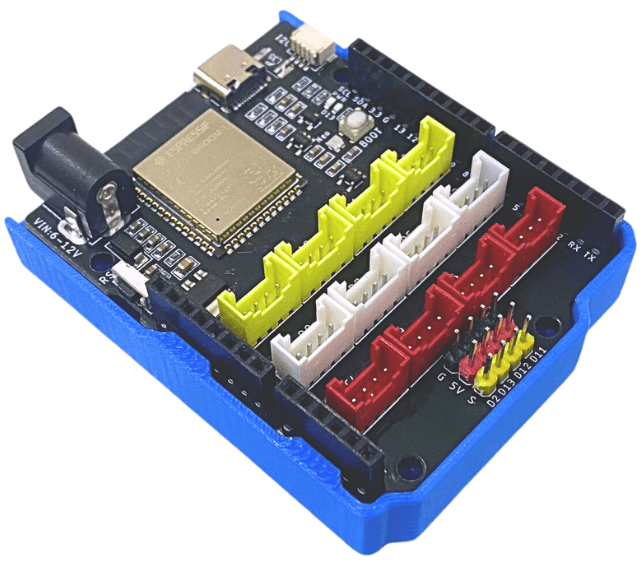
\includegraphics[width=0.5\textwidth]{SourceImage/yolo-uno.png}
    \caption{Board lập trình Yolo UNO và chip xử lý ESP32-S3}
    \label{fig:yolo_uno_board}
\end{figure}

\begin{table}[H]
    \centering
    \caption{Thông số kỹ thuật của board lập trình Yolo UNO trong hệ thống}
    \begin{tabular}{|l|l|}
    \hline
    \textbf{Thông số} & \textbf{Chi tiết} \\ \hline
    Vi xử lý & ESP32-S3 Dual Core 240MHz Tensilica Xtensa \\ \hline
    Bộ nhớ mở rộng & 16MB Flash, 8MB PSRAM \\ \hline
    Kết nối không dây & 2.4GHz Wi-Fi (802.11 b/g/n), Bluetooth 5.0, BLE \\ \hline
    Nguồn cấp hoạt động & 5VDC qua cổng USB Type-C hoặc Jack DC 5521 \\ \hline
    Nút nhấn tích hợp & Phím Reset, Phím chế độ Bootloader (BOOT0) \\ \hline
    Giao tiếp mở rộng & 12 cổng Grove (4 × Analog, 4 × Digital, 4 × I2C) \\ \hline
    Đèn hiển thị onboard & LED nguồn, LED chân D13, bóng LED RGB NeoPixel \\ \hline
    Chế độ cấu hình & Thiết lập chuẩn phần cứng 301B9 và 812H6 \\ \hline
    \end{tabular}
\end{table}

\subsubsection{Cảm biến nhiệt độ và độ ẩm DHT20}
DHT20 là dòng cảm biến nhiệt độ và độ ẩm kỹ thuật số thế hệ mới, được nâng cấp đáng kể so với các thế hệ trước. Cảm biến tích hợp chip ASIC cùng phần tử đo độ ẩm điện dung và đo nhiệt độ. DHT20 giao tiếp qua I2C, cho phép kết nối chung bus với các thiết bị I2C khác trên cùng bo mạch.

\begin{figure}[H]
    \centering
    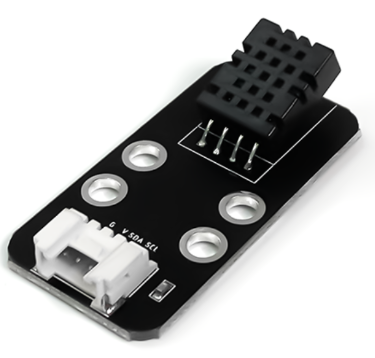
\includegraphics[width=0.4\textwidth]{SourceImage/DHT20 (1).png}
    \caption{Cảm biến nhiệt độ và độ ẩm kỹ thuật số I2C DHT20}
    \label{fig:sensor_dht20}
\end{figure}

\begin{table}[H]
    \centering
    \caption{Thông số kỹ thuật của cảm biến nhiệt độ và độ ẩm DHT20}
    \begin{tabular}{|l|l|}
    \hline
    \textbf{Thông số} & \textbf{Giá trị} \\ \hline
    Điện áp hoạt động & 2.2V -- 5.5V DC \\ \hline
    Giao thức truyền dữ liệu & I2C \\ \hline
    Phạm vi đo độ ẩm & 0\% -- 100\% RH \\ \hline
    Phạm vi đo nhiệt độ & -40$^{\circ}$C -- 80$^{\circ}$C \\ \hline
    Độ chính xác độ ẩm & $\pm$3\% RH \\ \hline
    Độ chính xác nhiệt độ & $\pm$0.5$^{\circ}$C \\ \hline
    \end{tabular}
\end{table}

\begin{table}[H]
    \centering
    \caption{Chức năng các chân kết nối của cảm biến DHT20}
    \begin{tabular}{|c|l|l|}
    \hline
    \textbf{STT} & \textbf{Chân} & \textbf{Chức năng} \\ \hline
    1 & VDD & Cấp nguồn dương (2.2V -- 5.5V) \\ \hline
    2 & SDA & Dây truyền nhận dữ liệu nối tiếp (Serial Data) \\ \hline
    3 & GND & Nối đất \\ \hline
    4 & SCL & Dây cấp xung nhịp nối tiếp (Serial Clock) \\ \hline
    \end{tabular}
\end{table}

\subsubsection{Đèn LED đơn cảnh báo (Tích hợp onboard)}
Trong dự án này, LED đơn được tích hợp sẵn trên bo mạch Yolo UNO, kết nối với GPIO~38. Binary Semaphore điều phối tần số nhấp nháy theo ba ngưỡng nhiệt độ.

\begin{table}[H]
    \centering
    \caption{Thông số kỹ thuật tiêu chuẩn của LED đơn cảnh báo}
    \begin{tabular}{|l|l|}
    \hline
    \textbf{Thông số} & \textbf{Giá trị} \\ \hline
    Điện áp kích hoạt thuận & 1.8V -- 2.2VDC (tùy thuộc màu sắc LED) \\ \hline
    Dòng điện hoạt động định mức & 10mA -- 20mA \\ \hline
    Dạng tín hiệu điều khiển & Kích hoạt mức logic (High/Low) hoặc xung PWM \\ \hline
    \end{tabular}
\end{table}

\subsubsection{Đèn LED màu NeoPixel WS2812B (Tích hợp onboard)}
NeoPixel WS2812B là LED RGB tích hợp chip điều khiển bên trong, cho phép điều khiển màu sắc từng pixel qua một dây tín hiệu số. Mỗi pixel nhận gói dữ liệu 24-bit, 8-bit cho mỗi kênh màu. NeoPixel cũng được tích hợp sẵn trên bo mạch Yolo UNO (GPIO~18), được dùng để hiển thị ba mức màu cảnh báo theo độ ẩm.

\begin{table}[H]
    \centering
    \caption{Thông số kỹ thuật của bóng LED màu NeoPixel onboard}
    \begin{tabular}{|l|l|}
    \hline
    \textbf{Thông số} & \textbf{Giá trị} \\ \hline
    Điện áp hoạt động cấp vào & 5VDC \\ \hline
    Kiểu IC điều khiển tích hợp & WS2812B \\ \hline
    Định dạng cấu trúc màu sắc & RGB 24-bit (16,7 triệu màu sắc) \\ \hline
    Tần số truyền nhận dữ liệu số & 800 Khz \\ \hline
    \end{tabular}
\end{table}

\subsubsection{Màn hình hiển thị LCD I2C}
Màn hình LCD 16$\times$2 hiển thị văn bản cục bộ trực tiếp trên thiết bị. Màn hình sử dụng giao tiếp I2C và kết nối vào cổng Grove I2C trên Yolo UNO qua cáp kết nối bốn dây (VCC, GND, SDA, SCL). Truy cập LCD được bảo vệ bằng Mutex để tránh xung đột bus I2C giữa các tác vụ, đồng thời hiển thị ba trạng thái cảnh báo.
\begin{figure}[H]
    \centering
    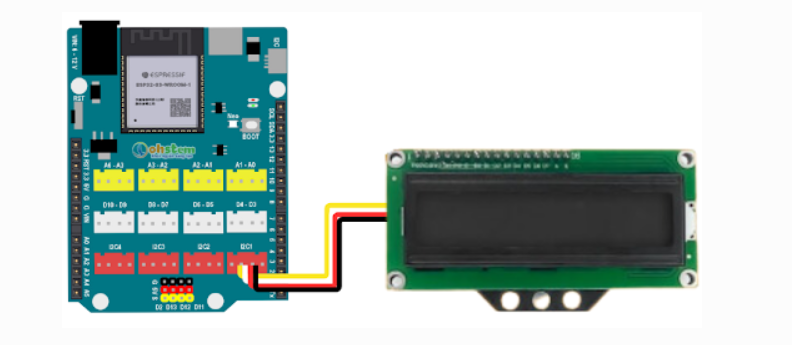
\includegraphics[width=0.9\textwidth]{SourceImage/LCD.png}
    \caption{Màn hình hiển thị LCD I2C cắm trực tiếp vào Yolo UNO qua cáp Grove}
    \label{fig:lcd_i2c}
\end{figure}
\begin{table}[H]
    \centering
    \caption{Thông số kỹ thuật của màn hình hiển thị LCD I2C}
    \begin{tabular}{|l|l|}
    \hline
    \textbf{Thông số} & \textbf{Giá trị} \\ \hline
    Điện áp hoạt động cấp vào & 5VDC \\ \hline
    Giao thức truyền dữ liệu chính & I2C \\ \hline
    Kết nối vật lý & Cáp 4 chân Grove (VCC, GND, SDA, SCL) \\ \hline
    Địa chỉ I2C mặc định & 0x27 hoặc 0x3F \\ \hline
    Đèn nền & Đèn LED tích hợp điều khiển qua phần mềm \\ \hline
    \end{tabular}
\end{table}
\begin{table}[H]
    \centering
    \caption{Chức năng các chân giao tiếp của màn hình LCD I2C}
    \begin{tabular}{|c|l|l|}
    \hline
    \textbf{STT} & \textbf{Chân} & \textbf{Chức năng} \\ \hline
    1 & GND & Nối đất \\ \hline
    2 & VCC & Cấp nguồn dương 5VDC \\ \hline
    3 & SDA & Dây truyền nhận dữ liệu nối tiếp (Serial Data) \\ \hline
    4 & SCL & Dây cấp xung nhịp nối tiếp (Serial Clock) \\ \hline
    \end{tabular}
\end{table}

\subsubsection{Giao thức truyền thông và kết nối}
Hệ thống IoT đòi hỏi sự linh hoạt trong cả truyền thông cục bộ cận biên lẫn truyền thông diện rộng lên máy chủ Internet:
\begin{itemize}
    \item \textbf{I2C:} Giao thức truyền thông nối tiếp, đồng bộ, hoạt động trên hai dây bus SDA và SCL. I2C hỗ trợ nhiều thiết bị trên cùng một bus nhờ cơ chế định địa chỉ, được dùng cho màn hình LCD và cảm biến DHT20.
    \item \textbf{Chuẩn kết nối Wi-Fi (IEEE 802.11):} Hoạt động trên dải tần 2.4GHz, đóng vai trò hạ tầng kết nối không dây chủ đạo của hệ thống nhúng. ESP32 S3 hỗ trợ cấu hình Wi-Fi linh hoạt bao gồm chế độ AP để thiết lập mạng cục bộ riêng biệt cho Web Server, và chế độ STA để lấy IP từ bộ định tuyến và thiết lập liên kết TCP/IP ra Internet.
    \item \textbf{Giao thức mạng HTTP, WebSocket và MQTT:} Phục vụ lớp ứng dụng trong kiến trúc IoT. Giao thức HTTP/WebSocket hoạt động theo mô hình truyền tải trực tiếp thích hợp cho Web Server và giao diện điều khiển (Dashboard) tại chỗ. MQTT hoạt động theo mô hình Publish-Subscribe gọn nhẹ, giảm thiểu băng thông đường truyền, tối ưu cho các tác vụ đẩy dữ liệu liên tục từ cảm biến lên đám mây Cloud.
\end{itemize}

\subsection{FreeRTOS}

\subsubsection{Quản lý tác vụ (Task Management)}
FreeRTOS là một hệ điều hành thời gian thực mã nguồn mở được thiết kế tối ưu cho vi điều khiển. Trong FreeRTOS, một ứng dụng được cấu thành từ nhiều tác vụ độc lập. Mỗi Task là một luồng thực thi riêng biệt sở hữu một không gian stack và mức độ ưu tiên được cấu hình độc lập tại thời điểm khởi tạo thông qua hàm \texttt{xTaskCreate()}. FreeRTOS quản lý vòng đời tác vụ qua bốn trạng thái: Running, Ready, Blocked và Suspended.

\subsubsection{Cơ chế lập lịch thời gian thực}
Bộ lập lịch của FreeRTOS đóng vai trò quyết định tác vụ nào ở trạng thái Ready sẽ được chuyển sang trạng thái Running. Hệ thống sử dụng thuật toán lập lịch ưu tiên có trưng dụng và chia sẻ thời gian. Hệ điều hành duy trì một bộ đếm xung nhịp hệ thống gọi là System Tick. Cứ sau mỗi chu kỳ Tick, Bộ lập lịch sẽ quét danh sách các tác vụ Ready; tác vụ nào có mức độ ưu tiên cao nhất sẽ giành quyền kiểm soát CPU (Context Switch). Nếu các tác vụ có mức độ ưu tiên bằng nhau, bộ lập lịch sẽ luân chuyển quyền thực thi theo Round-Robin.

\subsubsection{Giao tiếp và đồng bộ giữa các task}
Khi nhiều tác vụ chạy đồng thời và chia sẻ tài nguyên phần cứng (như bus I2C của LCD hoặc biến toàn cục), hiện tượng tranh chấp tài nguyên (Race Condition) rất dễ xảy ra nếu không có cơ chế đồng bộ hóa an toàn:
\begin{itemize}
    \item \textbf{Semaphore / Mutex:} Hoạt động theo cơ chế thẻ bài: Tác vụ muốn truy cập tài nguyên phải thực hiện hàm lấy thẻ (\texttt{xSemaphoreTake()}); nếu tài nguyên đang bận, tác vụ sẽ rơi vào trạng thái Blocked để nhường CPU cho tác vụ khác. Sau khi xử lý xong tài nguyên, tác vụ thực hiện giải phóng thẻ (\texttt{xSemaphoreGive()}). Dự án ứng dụng Semaphore và Mutex để đồng bộ hóa tác vụ cảnh báo LED, NeoPixel theo chu kỳ nhiệt độ/độ ẩm và điều phối quyền ghi dữ liệu lên LCD mà không dùng biến toàn cục.
    \item \textbf{Task Notifications:} Cơ chế truyền phát sự kiện trực tiếp đến một tác vụ cụ thể mà không cần qua các đối tượng trung gian. Việc sử dụng Task Notifications giải phóng đáng kể tài nguyên RAM và tối ưu hóa tốc độ chuyển đổi ngữ cảnh.
\end{itemize}

\subsubsection{Quản lý bộ nhớ}
FreeRTOS phân tách việc quản lý bộ nhớ thành hai vùng chính: bộ nhớ tĩnh (Static memory) và bộ nhớ động (Heap memory). FreeRTOS cung cấp nhiều mô hình quản lý bộ nhớ từ \texttt{heap\_1} đến \texttt{heap\_5}. Trong dự án phát triển IoT kết hợp TinyML, mô hình \texttt{heap\_4} thường được lựa chọn nhờ thuật toán gộp các khối bộ nhớ trống liền kề để giảm thiểu hiện tượng phân mảnh bộ nhớ, đảm bảo vùng nhớ cấp phát động cho các cấu trúc dữ liệu mạng luôn ổn định.

\subsubsection{Software Timer}
Software Timer cho phép thực thi một hàm callback sau một khoảng thời gian xác định, dựa trên System Tick mà không cần bộ định thời phần cứng. Timer có thể cấu hình ở chế độ One-shot hoặc Auto-reload, rất hữu ích cho các tác vụ định kỳ như quét trạng thái mạng Wi-Fi hoặc cập nhật thời gian hệ thống.

\subsubsection{Tiết kiệm năng lượng}
FreeRTOS hỗ trợ tính năng \texttt{configUSE\_IDLE\_HOOK} và chế độ Tickless Idle. Khi hệ thống nhận diện tất cả các tác vụ người dùng đều đang ở trạng thái Blocked và không có tác vụ nào sẵn sàng thực thi, bộ lập lịch sẽ chuyển sang Idle Task. Tại đây, vi điều khiển có thể được cấu hình để đưa vào các Light Sleep hoặc Deep Sleep, ngắt các xung nhịp ngoại vi không cần thiết và chỉ thức dậy khi có ngắt phần cứng hoặc khi bộ đếm thời gian chạm ngưỡng quy định.

\subsubsection{Khả năng mở rộng và tương thích}
Kiến trúc của FreeRTOS được thiết kế theo dạng mô-đun hóa cao, HAL độc lập giúp hệ điều hành dễ dàng tương thích và mở rộng trên nhiều dòng cấu trúc vi điều khiển khác nhau (từ lõi ARM Cortex-M cho đến kiến trúc Xtensa Tensilica dual-core của ESP32 S3). Điều này cho phép nhà phát triển dễ dàng tích hợp thêm các thư viện phần mềm bên thứ ba mà không phá vỡ cấu trúc lập lịch thời gian thực hiện có.

\subsubsection{Các thư viện hỗ trợ IoT}
FreeRTOS cung cấp bộ thư viện hỗ trợ IoT bao gồm: FreeRTOS-Plus-TCP cho tầng mạng, mbedTLS cho mã hóa dữ liệu, và các thư viện giao tiếp mạng tối ưu bộ nhớ stack, giúp thiết bị nhúng kết nối với Broker cục bộ hoặc máy chủ đám mây.

\subsection{CoreIOT}

\subsubsection{Các chức năng chính của CoreIOT}
CoreIOT là nền tảng đám mây IoT cung cấp dịch vụ thu thập, lưu trữ và hiển thị dữ liệu cảm biến theo thời gian thực. Các chức năng cốt lõi bao gồm:
\begin{itemize}
    \item Tiếp nhận và lưu trữ có cấu trúc các chuỗi dữ liệu thời gian thực gửi về từ thiết bị nhúng.
    \item Hỗ trợ cơ chế định danh, quản lý vòng đời và xác thực bảo mật thiết bị kết nối.
    \item Tích hợp hệ thống phân tích dữ liệu, tự động kích hoạt các kịch bản cảnh báo (E-mail, SMS, Webhook) khi thông số vượt ngưỡng.
\end{itemize}

\subsubsection{Kiến trúc hệ thống}
Kiến trúc của nền tảng CoreIOT được xây dựng dựa trên mô hình ba tầng chuẩn mô hình IoT đám mây:
\begin{enumerate}
    \item \textbf{Tầng kết nối:} Tiếp nhận dữ liệu từ thiết bị qua HTTP và MQTT.
    \item \textbf{Tầng lưu trữ:} Sử dụng cơ sở dữ liệu chuỗi thời gian để ghi dữ liệu cảm biến liên tục.
    \item \textbf{Tầng ứng dụng:} Cung cấp API REST và Dashboard để người dùng truy vấn và hiển thị dữ liệu.
\end{enumerate}

% \subsubsection{Đặc điểm nổi bật}
% CoreIOT hỗ trợ gói tin JSON thu gọn, cung cấp giao diện Dashboard kéo thả và Solution Template định cấu hình sẵn. Thiết bị xác thực với máy chủ bằng Device Token duy nhất.

\subsection{TinyML}

\subsubsection{Đặc điểm của TinyML}
TinyML là lĩnh vực kết hợp hệ thống nhúng và học máy, hướng tới việc thực thi các mô hình trực tiếp trên thiết bị có tài nguyên hạn chế (vài trăm kB RAM). Suy luận được thực thi cục bộ, giảm độ trễ và không phụ thuộc vào kết nối mạng.

\subsubsection{Kiến trúc hoạt động của TinyML}
Quy trình thực thi một kiến trúc TinyML trên thiết bị biên tuân thủ chặt chẽ các giai đoạn sau:
\begin{enumerate}
    \item \textbf{Thu thập dữ liệu:} Dữ liệu thô liên tục được trích xuất từ cảm biến với tần số lấy mẫu cố định.
    \item \textbf{Tiền xử lý và trích xuất đặc trưng:} Loại bỏ nhiễu tín hiệu. Tùy thuộc vào thiết kế mô hình, dữ liệu có thể được chuẩn hóa về khoảng $[0, 1]$ hoặc $[-1, 1]$, hoặc được nạp thẳng dưới dạng dữ liệu số thực gốc để tối ưu chu trình tính toán.
    \item \textbf{Suy luận:} Dữ liệu đặc trưng được đưa qua các lớp mạng nơ-ron (như CNN hoặc Dense Layers) để tính toán ma trận và đưa ra kết quả phân loại trạng thái. Để tăng tốc độ, mô hình có thể được lượng tử hóa hoặc giữ nguyên cấu trúc \texttt{float32}.
\end{enumerate}

\subsubsection{TensorFlow Lite Micro}
TensorFlow Lite Micro là framework học máy mã nguồn mở được thiết kế riêng bởi Google để chạy các mô hình học sâu trên các chip vi điều khiển kiến trúc 32-bit. Khung sườn này được tối ưu hóa triệt để để không sử dụng bất kỳ cơ chế cấp phát bộ nhớ động nào của hệ điều hành (không dùng \texttt{malloc} hay các toán tử \texttt{new}) nhằm tránh tuyệt đối lỗi phân mảnh RAM và đảm bảo tính thực thi an toàn cao. Toàn bộ các mảng trọng số, lớp mạng và biến trung gian của mô hình đều được quản lý tập trung trong một mảng bộ nhớ tĩnh được cấp phát từ trước gọi là \textbf{Tensor Arena}. Các toán tử tính toán trong thư viện được tối ưu hóa toán học để tận dụng tối đa tập lệnh phần cứng của chip xử lý, giúp tăng tốc độ nhân ma trận.

\subsubsection{Ứng dụng của TinyML trong IoT}
Trong các hệ thống IoT, TinyML phân tích dữ liệu ngay trên thiết bị thay vì gửi toàn bộ dữ liệu thô lên đám mây. Thiết bị chỉ truyền kết quả phân loại hoặc cảnh báo khi mô hình phát hiện sự kiện bất thường, giảm băng thông và năng lượng tiêu thụ.
